\subsection{Funktionen von \docdesk{}}
\docdesk{} ist eine Webanwendung, welche den Freigabe-Workflow im Unternehmen unterstützt.
Dokumente welche durch die vergebenen Berechtigungen für den Nutzer sichtbar sind,
können freigegeben, abgelehnt oder in einen digitalen Papierkorb gelegt werden.
Eine Bearbeitung von Dateien wie PDF ist hingegen nicht möglich, sodass keine Inhalte verändert oder Seiten entfernt oder hinzugefügt werden können.

Alle Dokumente werden dabei vom \acrshort{OPM} von \compart{} zentral im \doccollect{} verarbeitet und gesammelt.
Dabei werden alle Dokumente, für die keine Freigabe notwendig ist (nicht angefordert),
automatisch weitergeleitet bzw. exportiert an den \pilot{}, welcher bei der \mediserv{} den Druck steuert.
\subsubsection{Freigabe-Workflow}
\label{sec:approval-workflow-dd}
\begin{figure}[htbp]
    \centering
    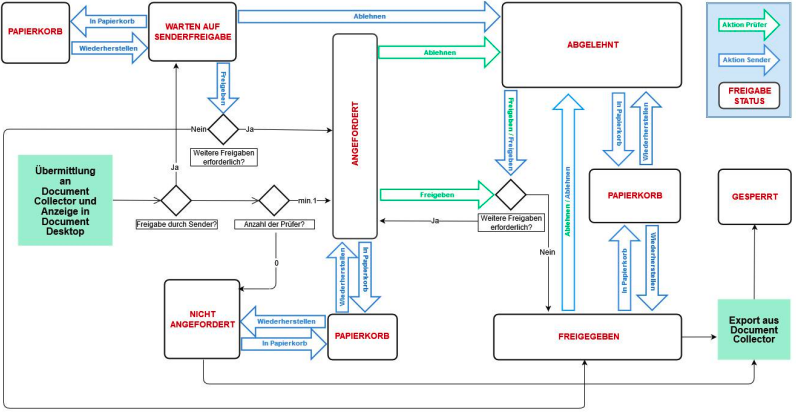
\includegraphics[width=\textwidth]{Freigabe-Workflow-DD.png}
    \caption{Freigabe Workflow in \docdesk{}}
    \label{fig:freigabe-workflow-dd}
\end{figure}

Alle Dokumente welche zu prüfen sind, erhalten den Status "`Angefordert"' und eine manuelle Prüfung ist notwendig.
Diese Dokumente können dann freigegeben oder abgelehnt werden.
Abgelehnte Dokumente können nicht weiterverarbeitet werden.
Ihr Status kann nur von der Person, welche den Status verändert hat, wieder freigegeben werden.
Wenn ein Dokument endgültig entfernt werden soll, wird dieses in den Papierkorb verschoben.
Endgültig werden die Dokumente aus dem Papierkorb entfernt, sobald diese manuell gelöscht werden oder das automatische Housekeeping die Daten aufräumt,
sprich diese nach einer festgelegten Zeit automatisch entfernt.
Bei vollständiger Freigabe werden die Dokumente ebenfalls in den \pilot{} exportiert.
Für jede Änderung des Dokumentenstatus ist es außerdem möglich, eine Notiz zu dieser hinzuzufügen,
welche zusätzliche Informationen über die Gründe für die Statusänderung gibt.
Diese können bereits mittels Templates vordefiniert werden, wobei diese Kommentare frei veränderbar sind.

Alle freigegeben Dokumente, welche exportiert sind, erhalten dabei den Status gesperrt und können nicht mehr verändert werden.
Eine grafische Darstellung des Freigabe-Prozesses lässt sich dabei \autoref{fig:freigabe-workflow-dd} entnehmen. \wholesection{compart_document_2020}{S. 1-6}

\subsubsection{Berechtigungskonzept und Filtermöglichkeiten}
Die Berechtigung zur Anzeige und Freigabe von Dokumenten im \docdesk{} erfolgt über die Zuordnung eines Benutzers zu Gruppen und damit Rollen.
Die Zugriffsberechtigungen gelten dabei immer für eine Kombination aus Mandant und Dokumentenklasse und werden über Zugriffskontrolllisten für die Rollen festgelegt.\vgl{compart_document_admin_2020}{S. 8, 9}
Der Mandant kann dabei der Repräsentation einer Organisationseinheit dienen. Dokumentenklassen fassen ähnliche Dokumente zu einer Gruppe zusammen.
Für jeden Mandanten können mehrere Dokumentenklassen definiert werden.
Über diese Auswahl werden die anzuzeigenden Dokumente bereits gefiltert, sodass nur die Dokumente aus der passenden Mandaten-Dokumentenklasse Kombination angezeigt werden.
Jedes Dokument hat zusätzliche Metadaten, welche z.T. von \compart{} vorgegeben sind und z.T. selbst konfiguriert werden können.
Dies kann z.~B. der Freigabestatus oder eine Vertragsnummer sein.
Über diese Metadaten können die Dokumente dann weiter eingeschränkt und gefiltert werden.\wholesection{compart_document_2020}{S. 5, 14}

\subsubsection{User Interface}
Da es sich bei dem \docdesk{} um eine Webanwendung handelt, wird diese im Browser geöffnet.
Zentral werden dabei alle Dokumente, welche der Kombination aus Mandant, Dokumentenklasse und Filterung entsprechen, in einer Tabelle angezeigt.
Diese kann durch den Nutzer entsprechend konfiguriert werden, um die benötigten Metadaten anzuzeigen.
Bei der Auswahl eines Dokumentes wird das dazugehörige PDF in einer Vorschau angezeigt,
welche auch durch eine Ansicht der Metadaten und den Verlauf des Dokuments ausgetauscht werden kann.
Mittels einer Checkbox werden bestimmte oder alle Dokumente ausgewählt, um sie freizugeben oder abzulehnen.
Ein Einblick in die UI liefert die \autoref{fig:hauptfenster-dd}.
\begin{figure}[htbp]
    \centering
    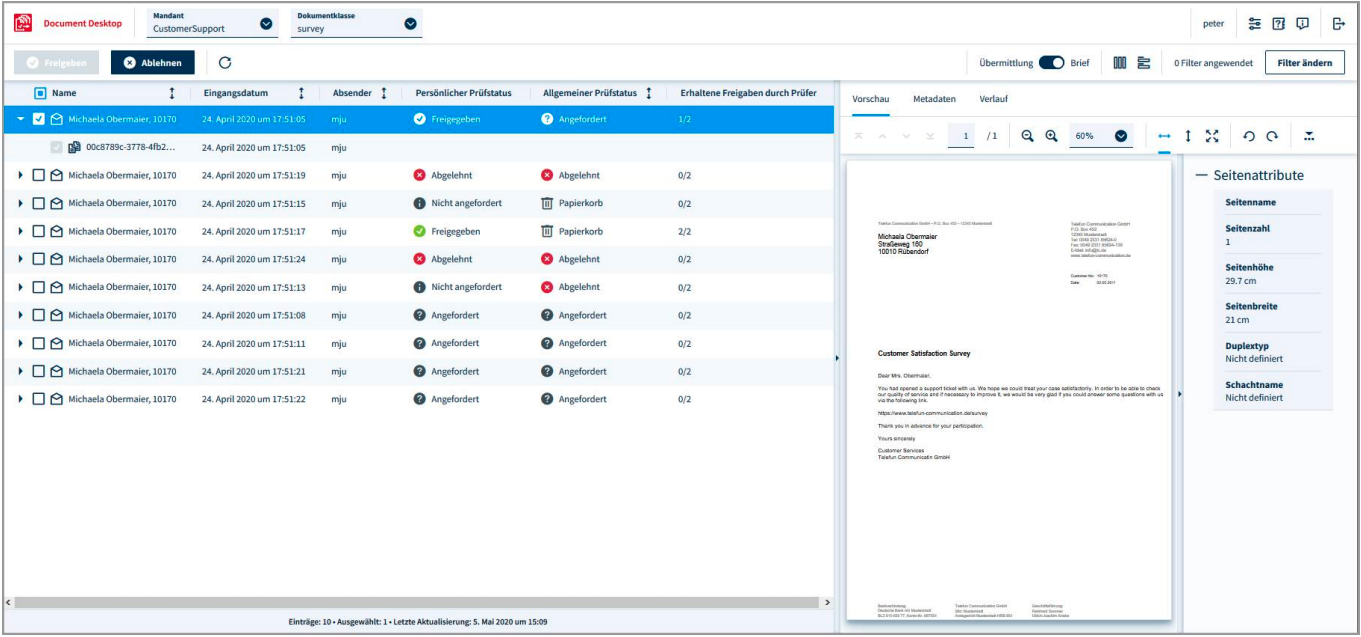
\includegraphics[width=\textwidth]{DD-Hauptfenster.png}
    \caption{Hauptfenster in \docdesk{}}
    \label{fig:hauptfenster-dd}
\end{figure}

\subsubsection{Administration und Konfiguration}
Der \docdesk{} wird wie die meisten Tools von \compart{} mittels XML Dateien konfiguriert.
In diesen werden die verschiedenen Mandanten, Dokumentenklassen, Gruppen und Rollen definiert.
Nutzer lassen sich entweder direkt innerhalb der Anwendungen anlegen,
es bestehen aber auch Schnittstellen zu LDAP und Active Directory.
Die Benutzer und Gruppen können dabei dann den passenden Gruppen im \docdesk{} zugeordnet werden.
Außerdem bietet der \docdesk{} eine \acrshort{REST}-\acrshort{API}, welche einige Funktionen zur Administration von Benutzern bietet.

Im \docdesk{} besteht auch die Möglichkeit mit anderer Software zu interagieren, beispielsweise mittels einer \acrshort{API}.
Auch Java-Script und Java stehen zur Verfügung um eigene Logiken einzubinden.
Dadurch besteht die Möglichkeit, den \docdesk{} hinsichtlich vor- oder nachgelagerter Prozesse an das eigene Unternehmen anzupassen.
Die Grundfunktionalität wie den \nameref{sec:approval-workflow-dd} mit den einzelnen Status kann dabei nicht verändert werden.
